\documentclass[../Notes.tex]{subfiles}
\usepackage{../Style/Diagrams}
\usepackage{../Style/Master}
\usepackage{../Style/boxes}
\usepackage{../Style/DefNoteFact}
\usepackage{../Style/QnsProof}
\usepackage{../Style/Thms}
\usepackage{../Style/Env}
\usepackage{../Style/NewCommands}
\begin{document}
\chapter{Continuous Random Variables}
\begin{stbox}{General Information}
  \begin{itemize}
    \item A function \(f \colon \mathbb{R}\to \mathbb{R}\) is a \emph{probability mass function} (pdf) of a continuous random variable \(X\) iff \(f\) is nonnegative and \(\int_{-\infty}^{\infty}f(x)\,dx=1\).
    \item For any probability mass function \(f\), we have \(\Prob(a\leq X\leq b)=\int_{a}^{b}f(x)\,dx\). Whether the inequality is strict or nonstrict does not affect the above identity. 
    \item A \emph{mode} of \(X\) is any value \(m\) such that \(f(m)\) is maximum.
    \item A \emph{cumulative distribution function} (cdf) \(F \colon \mathbb{R}\to [0,1]\) of a random variable \(X\) is defined by
    \[F(x):=P(X\leq x)=\int_{-\infty}^{x}f(x)\,dx.\]
    \item When writing out the cdf as a piecewise function, we explicitly write out the range of values for each case. We reserve the use of ``otherwise'' for pdf's.
    \item Any cdf is continuous and nondecreasing.
    \item Let \(X\) be a continuous random variable with cdf \(F\). To find the pdf \(g\) of any \(y(X)\), we first find its cdf, then differentiate. We achieve this by reverse engineering \(y(X)\leq y\) to find an inequality that relates \(X\) with \(y\). E.g. \(e^X\leq y\) iff \(X\leq \ln(y)\).
    \item A \emph{median} of \(X\) is any value \(m\) such that \(\Prob(X\leq m)=F(m)=1/2\).
    \item Mean/Expectation: 
    \[\mu=\E(X):=\int_{-\infty}^{\infty}xf(x)\,dx \qquad\text{and}\qquad \E(g(X))=\int_{-\infty}^{\infty}g(x)f(x)\,dx.\]
    \item Important property: 
    \[\E(ag(X)\pm bh(x))=a\E(g(X))\pm\E(h(X)).\]
    \item Variance: 
    \[\Var(X):=\E(X^2)-[\E(X)]^2.\]
    \item Important property:
    \[\Var(aX\pm b)=a^2\Var(X).\]
    \item A continuous random variable \(X\) has a \emph{uniform distribution} over the interval \([a,b]\) iff its pdf \(f\) is such that
    \[f(x)=\begin{cases}
      \frac{1}{b-a} &\text{if \(a<x<b\),}\\
      0 &\text{otherwise.}
    \end{cases}\] 
  \end{itemize}
\end{stbox}

\chapter{Special Continuous Random Variables}
\begin{definition}{}{}
  A continuous random variable \(X\) has a \emph{normal distribution} with mean \(\mu\) and standard deviation \(\sigma\), denoted by \(X \sim \operatorname{N}(\mu,\sigma^2)\), iff its pdf \(f\) is such that 
  \[f(x)=\frac{1}{\sigma\sqrt{2\pi}}\exp\left(-\frac{(x-\mu)^2}{2\sigma^2}\right).\]
\end{definition}
\begin{stbox}{General Information}
  \begin{enumerate}
    \item A normal distribution is symmetrical about the line \(x=\mu\). That is 
    \[\Prob(X\leq\mu-\delta)=\Prob(X\geq\mu+\delta)\]
    for each \(\delta>0\). Note that the mean, median, and mode coincide with \(\mu\).
    \item Properties of the normal distribution. Let \(X\) and \(Y\) be independent, such that \(X \sim \operatorname{N}(\mu,\sigma^2)\) and \(Y \sim \operatorname{N}(m,s^2)\). Then, for any \(n \in \mathbb{N}\) and \(x\), \(y \in \mathbb{R}\),  
    \begin{enumerate}
      \item \(nX \sim \operatorname{N}(n\mu,n^2\sigma^2)\),
      \item \(X_1+X_2+\cdots+X_n \sim \operatorname{N}(n\mu,n\sigma^2)\),
      \item \(aX\pm bY \sim \operatorname{N}(a\mu\pm bm,a^2\sigma^2+b^2s^2)\).
    \end{enumerate}
    \item A variable \(Z\sim \operatorname{N}(0,1)\) is said to follow the \emph{standard} normal distribution.

    \emph{Note}: \(Z\) is reserved for this purpose.
    \item Let \(X \in \operatorname{N}(\mu,\sigma^2)\). Then, \(\frac{X-\mu}{\sigma}\) follows the standard normal distribution. 
  \end{enumerate}
\end{stbox}

\chapter{Correlation and Linear Regression}
\begin{note}
  A good scatter diagram should follow the guidelines below.
  \begin{itemize}
    \item The relative position of each point on the scatter diagram should be clearly shown.
    \item The range of values for the set of data should be clearly shown by marking out the extreme \(x\) and \(y\) values on the corresponding axis.
    \item The axes should be labeled clearly with the variables.
  \end{itemize}
\end{note}
\begin{stbox}{General Information}
  \begin{itemize}
    \item The Product Moment Correlation Coefficient is a measure of the linear correlation between two variables. It is defined by
    \[r=\frac{\sum{(x-\bar{x})(y-\bar{y})}}{\sqrt{\sum{(x-\bar{x})^2}\sum{(y-\bar{y})^2}}}=\frac{\sum{xy}-\dfrac{\sum{x}\sum{y}}{n}}{\sqrt{\left[\sum{x^2}-\dfrac{\left(\sum{x}\right)^2}{n}\right]\left[\sum{y^2}-\dfrac{\left(\sum{y}\right)^2}{n}\right]}},\]
    which takes on a value from 0 to 1.
    \item When \(r=0\), there is no linear relationship. But, a nonlinear relationship may be present. Additionally, the regression lines are perpendicular.
    \item The closer the value of \(r\) is to 1 (or -1), the stronger the positive (or negative) linear correlation. Furthermore, the regression lines coincide.
    \begin{center}
      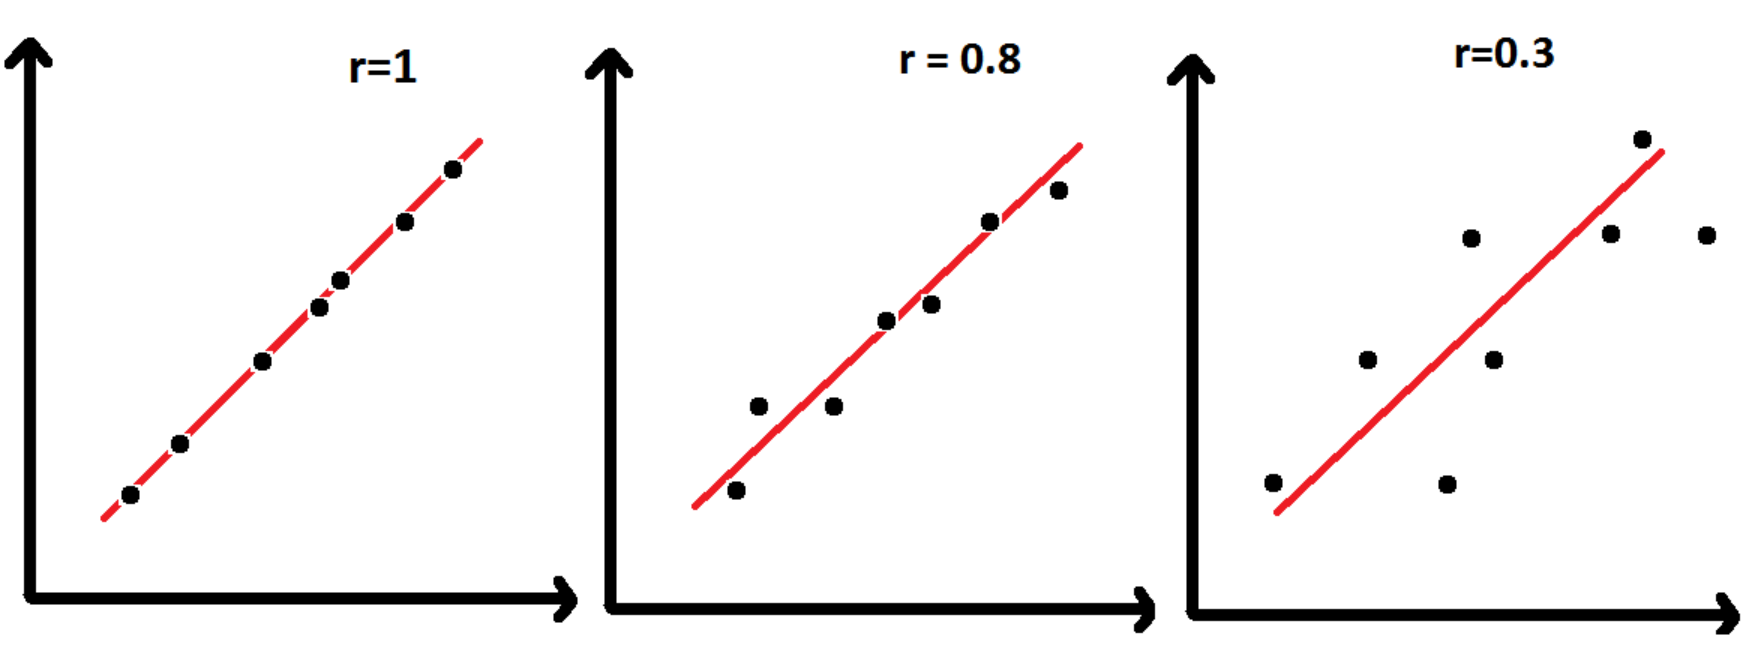
\includegraphics[scale=0.3]{../images/Product Moment Correlation Coefficient 1.png}
      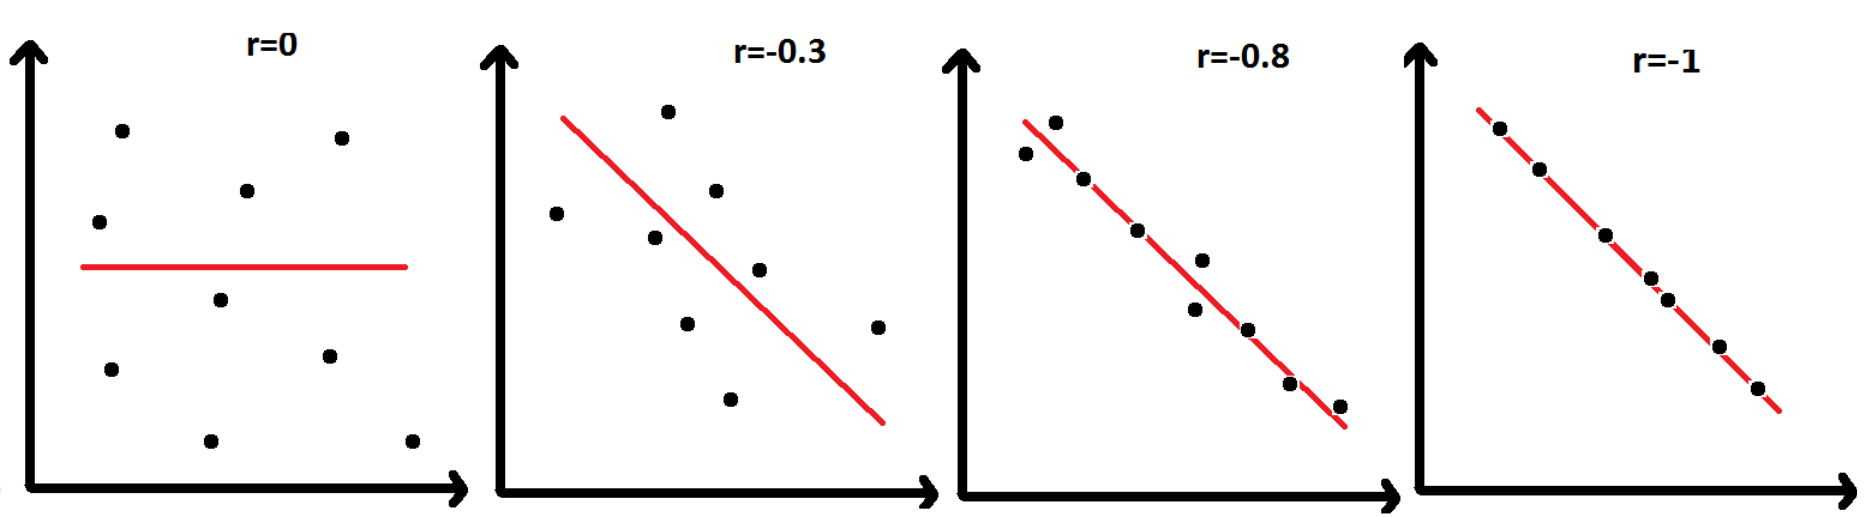
\includegraphics[scale=0.4]{../images/Product Moment Correlation Coefficient 2.png}
    \end{center}
    \item The regression line of \(y\) on \(x\) minimises the sum of squares deviation (error) in the \(y\)-direction. (i.e. we are assuming \(x\) is the independent variable whose values are known exactly.) It is given by
    \[y=\bar{y}+b(x-\bar{x}),\qquad\text{where}\qquad b=\frac{\sum{(x-\bar{x})(y-\bar{y})}}{\sum{(x-\bar{x})^2}}=\frac{\sum{xy}-\dfrac{\sum{x}\sum{y}}{n}}{\sum{x^2}-\dfrac{\left(\sum{x}\right)^2}{n}}.\] 
    \item The point \((\bar{x},\bar{y})\) always lies on both the regression lines of \(y\) on \(x\), and \(x\) on \(y\).
    \item Say we are given the value of one variable, and asked to approximate the the value of the other variable. Then, we should always use the line of the \emph{dependent} variable on the \emph{independent}.
    \item Estimations should not be taken for data outside the range of the sample provided, even if the value of \(r\) is close to 1.
  \end{itemize}
\end{stbox}
\end{document}